\documentclass[a4paper,12pt,fleqn]{scrartcl}%fleqn pour aligner les equations à gauche
\usepackage{../../Styles/Exercice}


\newcommand{\chnum}{Chapitre 13}
\newcommand{\chtitle}{Mouvement des astres et des planètes}
\newcommand{\dtype}{Exercices}
  
  
\begin{document}
\maketitle

\begin{multicols}{2}
\section{Astéroïde Théa Sylvia II Rémus - 2005}
On s'intéresse à l'astéroïde Rhéa Sylvia décrivant une orbite elliptique autour du Soleil selon le schéma ci-contre.
	\begin{center}
	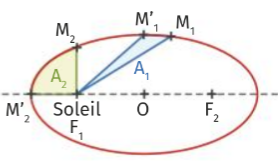
\includegraphics[width=.8\linewidth]{Ressources/TSPE_C6_Ex_Fig1.png}
	\end{center}
\begin{enumerate}
	\item Justifier la position du Soleil indiquée sur le schéma ci-dessus en cotant la loi de Kepler utilisée.
	\item On suppose que les durées de parcours entre les points $M_1$ et $M_1'$, puis $M_2$ et $M_2'$ sont égales. En utilisant une des lois de Kepler, donner la relation existante entre les aires $A_1$ et $A_2$.
\end{enumerate}

\section{Rencontre de la sonde Cassini avec Saturne}
Lors de sa mission d'exploration, la sonde européenne Cassini-Huygens a livré les premiers clichés de Saturne, noté S, de ses anneaux et de ses nombreux satellites dont Titan, noté T, le plus grand, de masse $M$. On considérera que son centre décrit une trajectoire circulaire autour de Saturne.
\begin{enumerate}
	\item Représenter qualitativement sur un schéma Saturne, Titan et la force de gravitation appliquée sur Titan.
	\item Donner l'expression vectorielle de cette force.
	\item Exprimer l'accélération vectorielle de Titan en précisant la loi utilisée. Préciser ses caractéristiques.
	\item Montrer que le mouvement de Titan est uniforme.
	\item Montrer que l'expression de la vitesse orbitale de Titan autour de Saturne est $v_T = \sqrt{\dfrac{G \cdot M_S}{r_T}}$. Calculer sa valeur.
\end{enumerate}
\begin{data}
\begin{itemize*}
	\item \textbf{Constante de gravitation universelle :} $G$ = \SI{6,67E-11}{ \meter \cubed \per \kilo \gram \per \second \squared}
	\item \textbf{Rayon de l'orbite de Titan :} $r_T$ = \SI{1,22E6}{\kilo \meter}
	\item \textbf{Rayon de Saturne :} $R_S$ = \SI{5,8E4}{\kilo \meter}
	\item \textbf{Masse de Saturne :} $M_S$ = \SI{5,69E26}{\kilo \gram}
\end{itemize*}
\end{data}

\section{Alphasat, satellite géostationnaire européen}
Le satellite Alphasat a été mis en orbite géostationnaire par la société Arianespace depuis Kourou en 2013. Il a pour but d'assurer des missions de télécommunications. Il se déplace suivant une trajectoire supposée circulaire de rayon $r$ et possède une masse $m$.
\begin{enumerate}
	\item Expliquer ce qu'est un satellite géostationnaire.
	\item Préciser le référentiel le plus adapté pour étudier le mouvement du satellite, assimilé à un point ponctuel $S$.
	\item Dans le repère de Frenet, retrouver l'expression du vecteur accélération $\vec{a_S}$ de $S$ tel que sa valeur est égale à $a_s=G \cdot \dfrac{M_T}{r^2}$
\end{enumerate}



\section{Trajectoire d'une comète}
\begin{minipage}{.5\textwidth}
La trajectoire d'une comète est tracée ci-dessous dans le référentiel héliocentrique. On suppose que les durées  de parcours entre les points $M_1$ et $M_1'$, puis $M_2$ et $M_2'$ sont égales. La comète est soumise à l'attraction gravitationnelle du Soleil. Toute autre attraction est négligeable.\\
\end{minipage}
\begin{minipage}{.5\textwidth}
	\begin{center}
	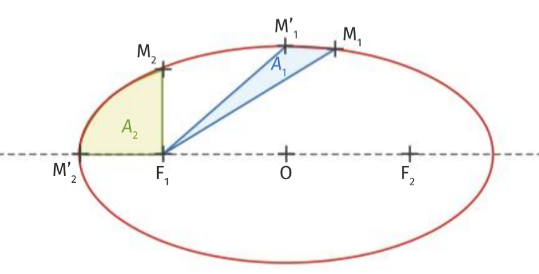
\includegraphics[width=.8\linewidth]{Ressources/TSPE_C6_Ex_Fig3.png}
	\end{center}
\end{minipage}
\begin{enumerate}
	\item Après avoir identifié la forme de la trajectoire, préciser ce que représentent les points $F_1$, $F_2$ et $O$.
	\item Déterminer sur quel parcours entre $M_1M_1'$ ou $M_2M_2'$ la vitesse de la comète est la plus importante. Expliquer.
	\item Représenter la force d'interaction gravitationnelle exercée sur la comète sur un point de la trajectoire
\end{enumerate}



\section{Couchers de soleils dur Tatooine}

Dans la saga \textit{Star Wars}, Tatooine a la particularité d'être en orbite autour de deux étoiles Tatoo 1 et Tatoo 2. Du point de vue de la planète, tout se passe comme si les étoiles n'en faisaient qu'une. On peut estimer que leur distance est légèrement supérieure à 10 millions de kilomètres. En vérité, pour ne pas être inhabitable et expliquer son aspect désertique, une bonne position de Tatooine serait de deux cents millions de kilomètres.
\begin{center}
	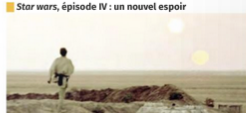
\includegraphics[width=\linewidth]{Ressources/TSPE_C6_Ex_Fig4.png}
\end{center}
\begin{enumerate}
	\item En supposant que Tatoo 1 et Tatoo 2 sont à égale distance de Tatooine, montrer, en s'appuyant sur la photo et sur le texte, que la valeur du rayon de chacune des deux étoiles est environ égale à deux millions de kilomètres.
	\item En supposant que les étoiles possèdent la même masse volumique que le Soleil, évaluer leur masse.
\end{enumerate}
On estime pour la suite que la masse des deux étoiles est égale à $M_{tatoo}$ = \SI{9,3E31}{\kilo \gram}.
\begin{enumerate}[resume]
	\item Faire un schéma du système Tatooine-Tatoo$_{1-2}$ et représenter sans soucis d'échelle la force d'attraction gravitationnelle exercée par Tatoo$_{1-2}$ sur Tatooine ainsi que le vecteur accélération de Tatooine.
	\item Montrer que le mouvement, supposé circulaire, de la planète dans ce référentiel est uniforme.
	\item Déterminer la période de révolution de Tatooine. Conclure.
\end{enumerate}
\begin{data}
\begin{itemize*}
	\item \textbf{Rayon :} $R_{Soleil}$ = \SI{7,0E5}{\kilo \meter}
	\item \textbf{Masse :} $M_{Soleil}$ = \SI{2,0E30}{\kilo \gram}
	\item \textbf{Volume d'une sphère de rayon $r$ :} $V=\dfrac{4}{3}\pi \cdot r^3$
\end{itemize*}
\end{data}
\end{multicols}
\end{document}